\subsubsection{Caso d'uso UC4.1:  Login Base}
\label{UC4_1}
\begin{figure}[ht]
	\centering
	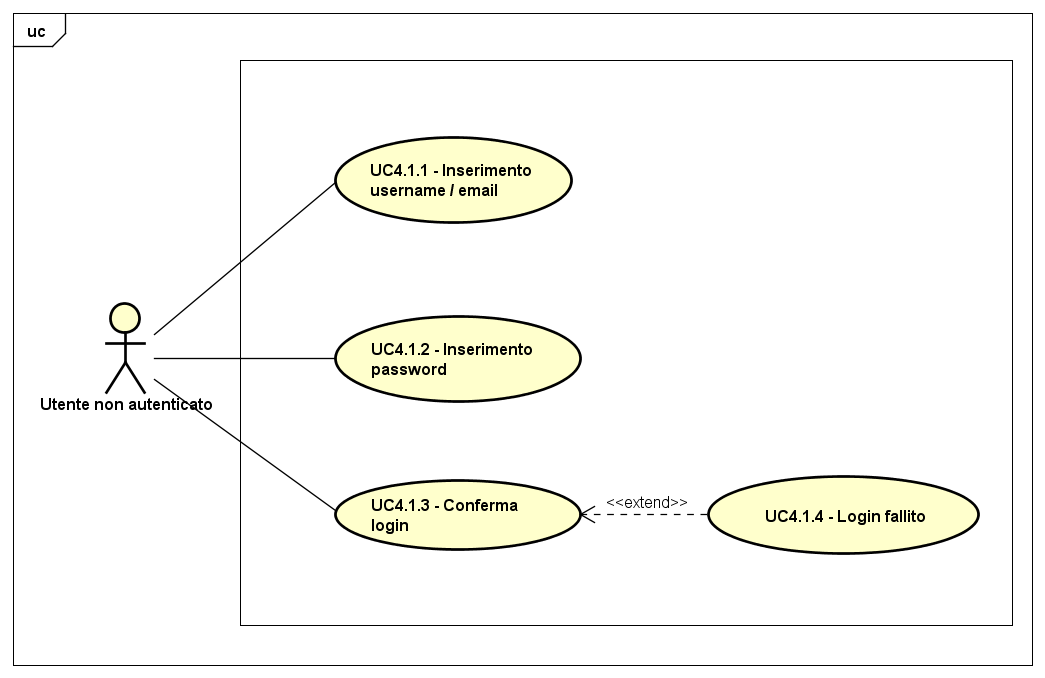
\includegraphics[scale=0.45]{UML/UC4_1.png}
	\caption{UC4.1: Login Base}
\end{figure}

\begin{tabular}{ l | p{11cm}}
	\hline
	\rowcolor{Gray}
	 \multicolumn{2}{c}{UC4.1 - Login Base} \\
	 \hline
	\textbf{Attori} & Utente Non Autenticato \\
	\textbf{Descrizione} & L'utente non autenticato effettua il login all'applicazione web, così da evolversi in un utente autenticato\\
	\textbf{Pre-Condizioni} & L'utente ha scelto di eseguire il login all'applicazione web e non è autenticato \\
	\textbf{Post-Condizioni} & L'utente ha effettuato il login all'applicazione web, evolvendosi in un utente autenticato \\
	\textbf{Scenario Principale} & 
	\begin{enumerate*}[label=(\arabic*.),itemjoin={\newline}]
		\item L'utente non autenticato può inserire l'email o username(UC4.1.1)
		\item L'utente non autenticato può inserire la password(UC4.1.2)
		\item L'utente non autenticato può confermare i dati per loggarsi(UC4.1.3)
	\end{enumerate*}\\
		\textbf{Scenari Alternativi} & 
	\begin{enumerate*}[label=(\arabic*.),itemjoin={\newline}]
		\item L'utente non autenticato visualizza un errore dovuto a un mismatch dei dati immessi e il login non avviene (UC4.1.4)
	\end{enumerate*}\\
\end{tabular}